\chapter{Performance Evaluation} \label{ch:evaluation}
\section{Evaluation in Controlled Environment}
The counting device was firstly mounted at a household doorframe to test its accuracy. The mounting height was about 2 meters and the ambient temperature was around $24^\circ C$. In a 40 minutes test, a test person was asked to enter and exit the room continuously for 100 times. The user interface shown in \autoref{fig:noderedui} was turned on in a smartphone so that the test person can read the algorithm output immediately.

The algorithm detects 94 enter events correctly and 97 exit events correctly. And it has successfully handled multiple-human events, such as sequential entering and passing in opposite directions.
\section{Evaluation in Uncontrolled Environment}
The counting device has also been attached to the ceiling of the main entrance in our faculty department to evaluate its performance in real situations. The mounting height was a little higher than the previous experiment, at about 3 meters. The device has operated for two weeks around the clock, except for the first 2 days in the second week because of a local network update. The device transmits the counting result of the proposed algorithm as well as the actual infrared image for later annotation. By this way, we have collected a valid dataset of 8 days in total. The evaluation time slot begins from 8:00 in the morning and ends at 20:00.

The ground truth is annotated by manually iterating through all received images. For ease of examination, the device has only transmitted images when there are three pixels hotter than ambient temperature. Usually, the image transmission begins when a human enters the camera FOV and terminates when the human leaves. We regard each video sequence as one individual event (or two closely happening events). A timestamp was attached to each video sequence to indicate the time of that event. By this way, the number of images to be reviewed is reduced from several hundreds of thousands to a moderate number of around one thousand.

The manual ground truth annotation can only locate the time of event occurrence to minutes. However, the counting algorithm outputs an accurate millisecond timestamp when the count changes. This time disparity in timestamp has caused difficulty in matching the ground truth and the algorithm output with automatic tools. Therefore the accuracy evaluation is carried out visually. For every ground truth enter or exit event, it is checked if the counting algorithm outputs a correct result (+1 for entering and -1 for exiting) in the nearby 30 seconds. If this is the case we add one to the correct counting category otherwise to the wrong counting category. A false detection, when no event is observed in the ground truth video sequence but the algorithm outputs a non-zero value, also falls into the wrong counting category. See \autoref{fig:ESKibana} for example, the event around 12:00 is a false detection and the event around 14:00 is a wrong counting, both will increase the number of ``wrong counting'' by one.

We have also picked out those events which involve multiple humans entering or exiting simultaneously and evaluated them separately. For such events, correct counting consists of the correct movement direction as well as the correct counting number. The counting of a multiple-human event is only regarded correct when the algorithm outputs the exact human number as observed in the ground truth. Take \autoref{fig:ESKibana} as an example, the long green bar plots around 11:20 and 16:00 are two correctly counted multiple-human events, and the events around 13:00 and 14:00 are wrong counting. Note that sometimes the algorithm outputs ``+2'' and two single entering events are observed at that time point, we regard such events as correctly counted.

The dataset statics are shown in \autoref{tab:eva_data}, all data are grouped in 2-hour time ranges. We have finally counted 222 correct and 50 wrong outputs in single human events, which amounts to an accuracy of 81.6\%. There have also been 10 correct and 6 wrong outputs in multiple-human events, which amounts to an accuracy of 62.5\%. The overall accuracy is around 80\%.

\begin{table}[]
\small
\begin{tabular}{l|ll|ll|l|ll|ll|}
\cline{2-5} \cline{7-10}
                            & \multicolumn{2}{l|}{single-human event} & \multicolumn{2}{l|}{multi-humans event} &       & \multicolumn{2}{l|}{single-human event} & \multicolumn{2}{l|}{multi-humans event} \\ \hline
\multicolumn{1}{|l|}{Day1}  & correct             & wrong             & correct             & wrong             & Day2  & correct             & wrong             & correct             & wrong             \\ \hline
\multicolumn{1}{|l|}{8:00}  & -                   & -                 & -                   & -                 & 8:00  & 5                   & 1                 & -                   & -                 \\
\multicolumn{1}{|l|}{10:00} & -                   & -                 & -                   & -                 & 10:00 & 10                  & 4                 & 1                   & 0                 \\
\multicolumn{1}{|l|}{12:00} & 9                   & 1                 & -                   & -                 & 12:00 & 11                  & 1                 & 0                   & 2                 \\
\multicolumn{1}{|l|}{14:00} & 4                   & 0                 & 1                   & 0                 & 14:00 & 24                  & 5                 & 1                   & 1                 \\
\multicolumn{1}{|l|}{16:00} & 5                   & 0                 & 0                   & 1                 & 16:00 & 9                   & -                 & -                   & -                 \\
\multicolumn{1}{|l|}{18:00} & 5                   & 1                 & -                   & -                 & 18:00 & -                   & -                 & -                   & -                 \\ \hline
\multicolumn{1}{|l|}{Day3}  & correct             & wrong             & correct             & wrong             & Day4  & correct             & wrong             & correct             & wrong             \\ \hline
\multicolumn{1}{|l|}{8:00}  & 8                   & 2                 & -                   & -                 & 8:00  & -                   & -                 & -                   & -                 \\
\multicolumn{1}{|l|}{10:00} & 5                   & 1                 & -                   & -                 & 10:00 & -                   & 1                 & -                   & -                 \\
\multicolumn{1}{|l|}{12:00} & 0                   & 1                 & 0                   & 1                 & 12:00 & 1                   & 1                 & -                   & -                 \\
\multicolumn{1}{|l|}{14:00} & 2                   & 0                 & 2                   & 0                 & 14:00 & 5                   & 2                 & -                   & -                 \\
\multicolumn{1}{|l|}{16:00} & 2                   & 0                 & -                   & -                 & 16:00 & 2                   & 1                 & 3                   & 0                 \\
\multicolumn{1}{|l|}{18:00} & -                   & -                 & -                   & -                 & 18:00 & -                   & -                 & -                   & -                 \\ \hline
\multicolumn{1}{|l|}{Day5}  & correct             & wrong             & correct             & wrong             & Day6  & correct             & wrong             & correct             & wrong             \\ \hline
\multicolumn{1}{|l|}{8:00}  & -                   & -                 & -                   & -                 & 8:00  & 7                   & 1                 & -                   & -                 \\
\multicolumn{1}{|l|}{10:00} & 0                   & 3                 & 0                   & 1                 & 10:00 & 1                   & 0                 & -                   & -                 \\
\multicolumn{1}{|l|}{12:00} & 7                   & 4                 & -                   & -                 & 12:00 & 6                   & 1                 & -                   & -                 \\
\multicolumn{1}{|l|}{14:00} & 7                   & 0                 & 1                   & 0                 & 14:00 & 8                   & 1                 & -                   & -                 \\
\multicolumn{1}{|l|}{16:00} & -                   & -                 & -                   & -                 & 16:00 & 4                   & 0                 & -                   & -                 \\
\multicolumn{1}{|l|}{18:00} & -                   & -                 & -                   & -                 & 18:00 & 3                   & 1                 & -                   & -                 \\ \hline
\multicolumn{1}{|l|}{Day7}  & correct             & wrong             & correct             & wrong             & Day8  & correct             & wrong             & correct             & wrong             \\ \hline
\multicolumn{1}{|l|}{8:00}  & -                   & -                 & -                   & -                 & 8:00  & 2                   & 0                 & -                   & -                 \\
\multicolumn{1}{|l|}{10:00} & 1                   & 3                 & -                   & -                 & 10:00 & 2                   & 0                 & -                   & -                 \\
\multicolumn{1}{|l|}{12:00} & 9                   & 1                 & -                   & -                 & 12:00 & 5                   & 1                 & -                   & -                 \\
\multicolumn{1}{|l|}{14:00} & 9                   & 2                 & 1                   & 0                 & 14:00 & 13                  & 3                 & -                   & -                 \\
\multicolumn{1}{|l|}{16:00} & 8                   & 3                 & -                   & -                 & 16:00 & 18                  & 3                 & -                   & -                 \\
\multicolumn{1}{|l|}{18:00} & 4                   & 1                 & -                   & -                 & 18:00 & 1                   & 0                 & -                   & -                 \\ \hline
\end{tabular}
\caption{Dataset statistics. The "-" symbol means entry is not applicable.}\label{tab:eva_data}
\end{table}

\section{Discussion}
To investigate what has caused the performance drop in the real situation, the observed possible issues have been categorized into five classes. And they are:
\begin{enumerate}
  \item Not detected: when a hot object is observed in the ground truth but the algorithm does not respond at all.
  \item Noise: when there is only random temperature fluctuation in the scene but the algorithm reports an object entering or leaving.
  \item Long sequence: when a human stands beneath the camera for a long period (several minutes).
  \item Heat disturbance: when the background temperature is not homogenous in the whole scene, for example, half of the FOV monitoring the sunny side of a doorway has a higher temperature.
  \item Missing frame: when somehow a few frames in a video sequence is not captured, which causes an abrupt position change of the detected object.
\end{enumerate}
\autoref{fig:eva_errors} shows the occurrence frequency of the aforementioned issues. Among which the ``missing frame'' error turned out to be the most common but also the most devastating issue that drastically reduced the accuracy of the proposed algorithm.
\begin{figure}
  \centering
  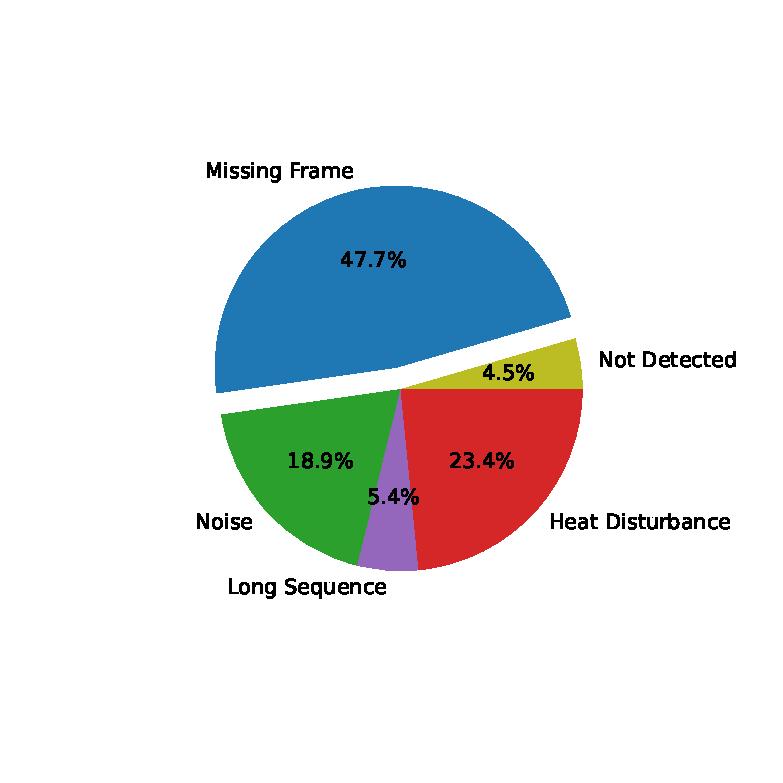
\includegraphics[width=0.6\textwidth]{figures/errors.eps}
  \caption{The percentage distribution of issues that may cause a detection or tracking failure.}\label{fig:eva_errors}
\end{figure}

\subsection{Missing Frame Error}
\begin{figure}
  \centering
  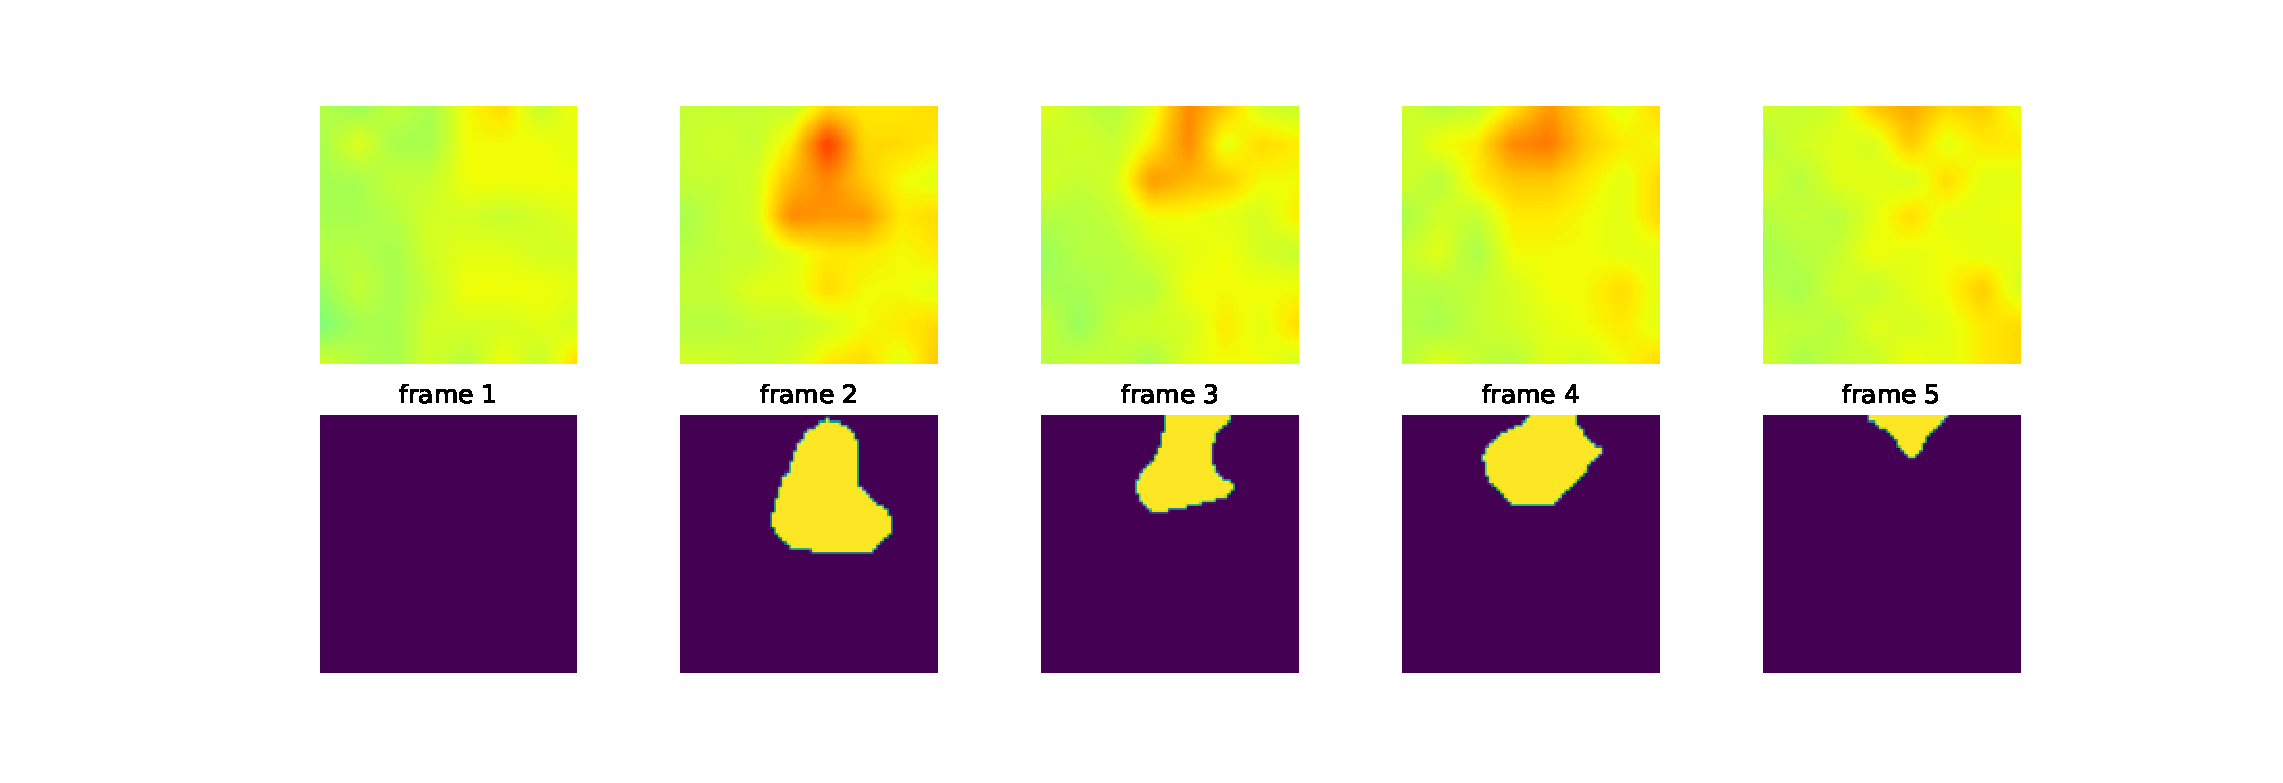
\includegraphics[width=\textwidth]{figures/err_missingframe.eps}
  \caption{This example shows an exit event where only the last few frames are captured, the missing frames of the event beginning makes it impossible to track and count the event correctly. The first row is the IR camera readings and the second row is the object mask.}\label{fig:err_mf}
\end{figure}
\autoref{fig:err_mf} demonstrates a typical detection failure that several beginning frames of an event are missed out. A further investigation shows this issue may be traced back to a network lagging. As mentioned in \Cref{ch:platform}, all the messages from the microcontroller are transmitted through a public MQTT broker so that realtime feedback can be obtained by running a listener client elsewhere. As contrary, in the controlled environment, both message publisher and listener locate under the same network and a local MQTT broker is used. Sending the messages to the Internet must have taken more time. Most of the message content is the raw IR image, which takes around 320 bytes. At a frame rate of 10 fps (when a human is detected), the generated data flow is about 3.5KB per second. Though the amount of data is still quite trivial, it is already larger than a common IoT application. Considering we use a public broker and the broker provider may have restrictions in the data amount, the network connection may deteriorate and finally cause a pause in the processing loop.

Moreover, the structure of the program could be improved. In the initial design, the message sending function is called within the tracking algorithm. Because it is observed that sending an image takes no longer than several milliseconds and will not break the time restriction for realtime processing. However, providing that a message sending may take several tens of milliseconds, the publishing task should be offloaded from the tracking algorithm. The task could be handled by another thread or even by the other CPU core. \autoref{fig:err_processloop} shows the improved program structure.
\begin{figure}
  \centering
    \subfloat[\centering the initial process loop]{{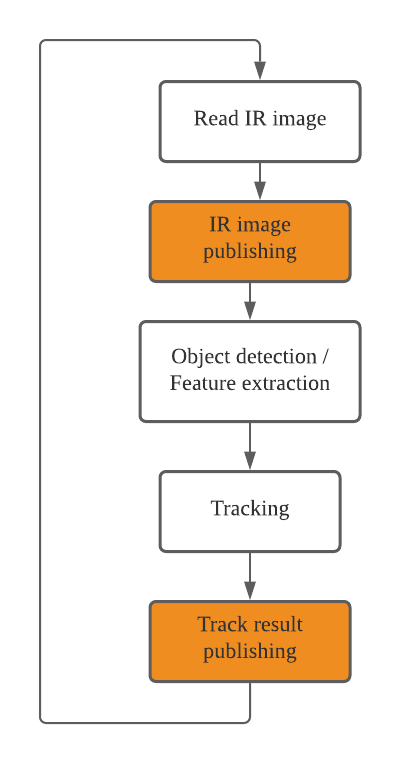
\includegraphics[width=0.3\textwidth]{figures/processloop1.png}}}%
    \qquad
    \subfloat[\centering the improved process loop]{{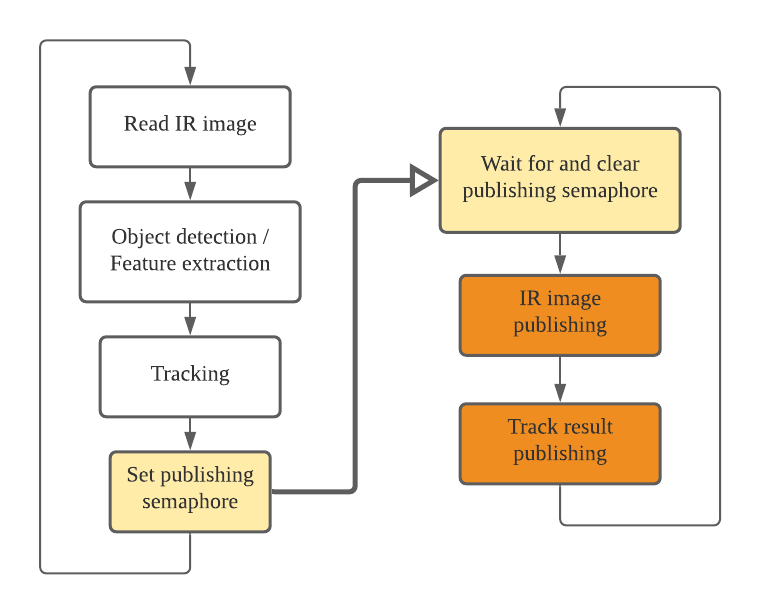
\includegraphics[width=0.6\textwidth]{figures/processloop2.png}}}%
    \caption{Initial and improved program flow. The orange blocks denote the time-consuming publishing tasks.}%
    \label{fig:err_processloop}
\end{figure}

After switching to a more stable broker, the number of missing frame error has reduced by 40\% (from 33 to 20). A lower error rate is expected when the publishing task is excluded from the process loop. Switching to a local broker instead of a public broker may also improve the network connection. Eventually, the image publishing task can be canceled totally because it is not needed in the deployment.

\subsection{Heat Disturbance Error}
\begin{figure}
  \centering
  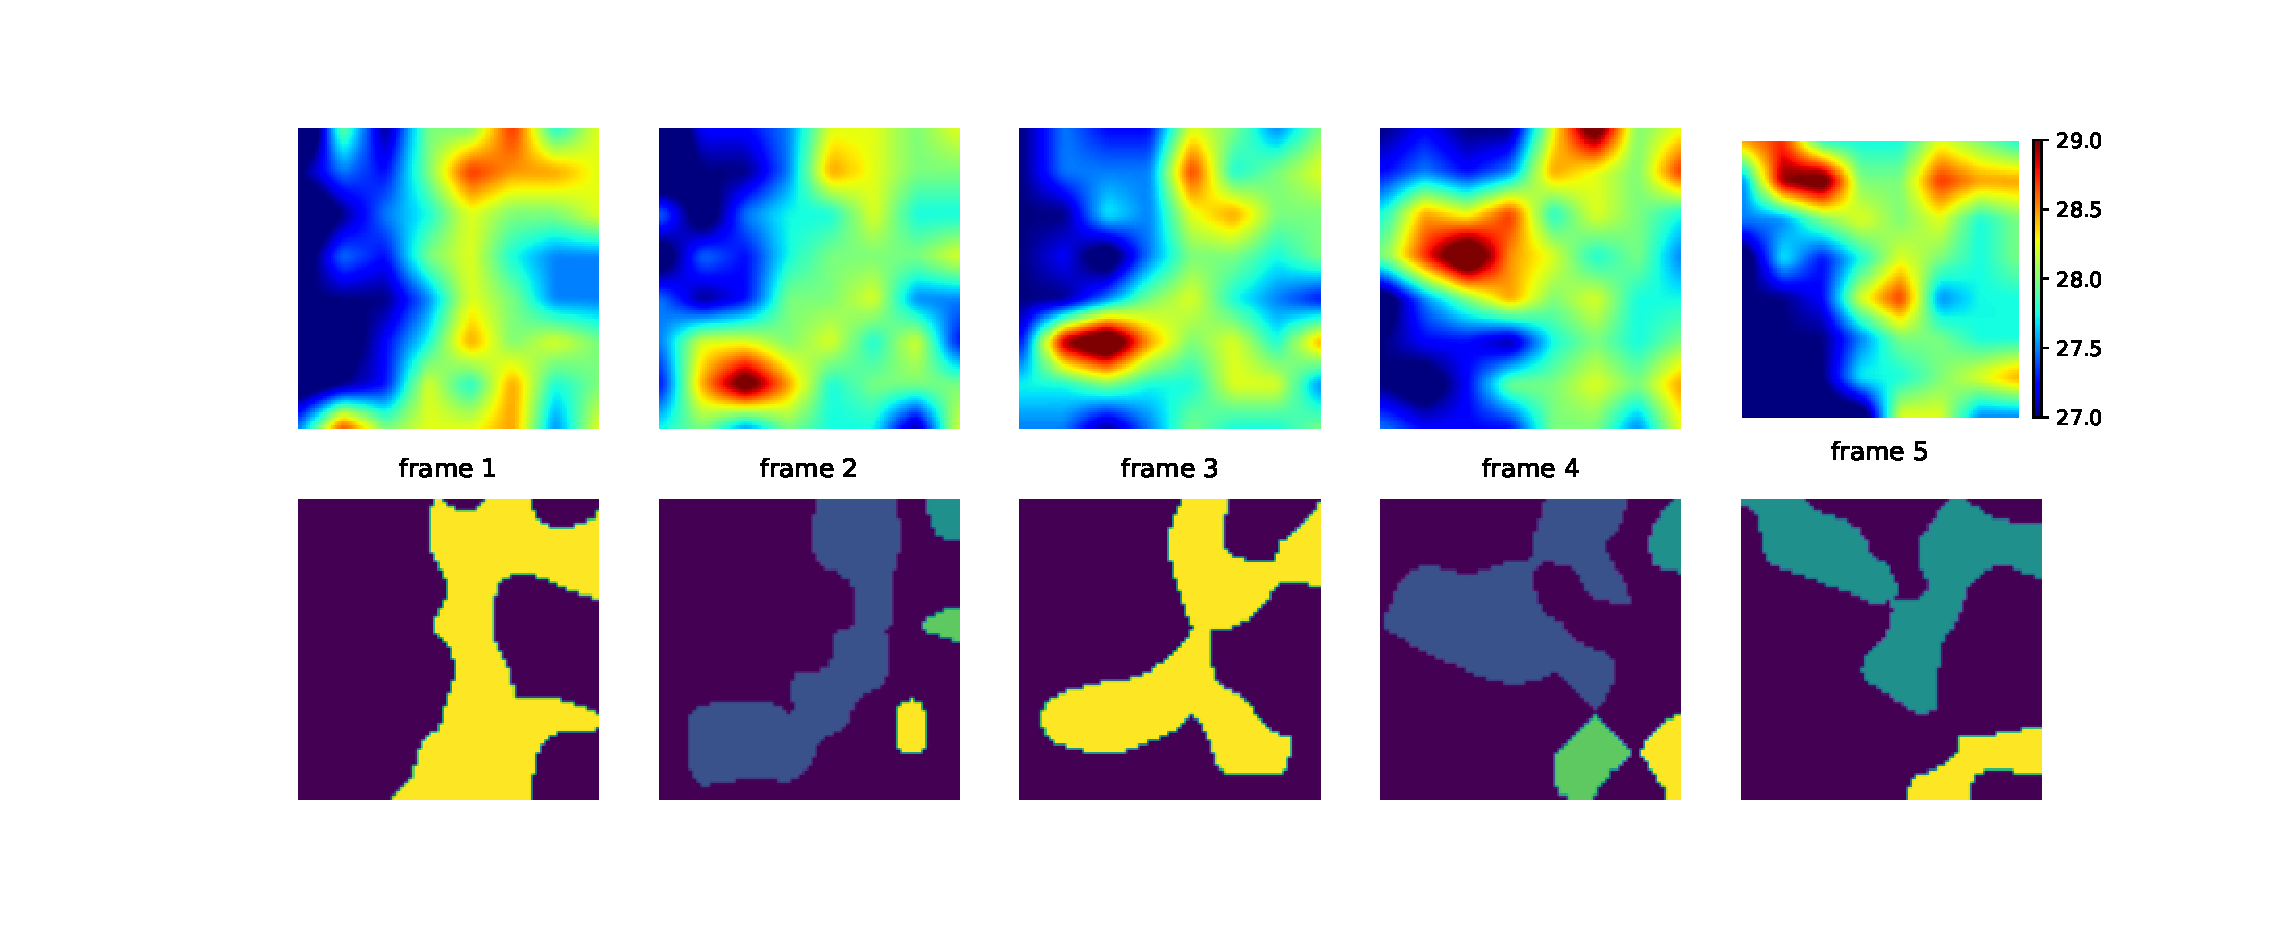
\includegraphics[width=\textwidth]{figures/err_heatdisturb.eps}
  \caption{This example shows a human leaving the room (on the left side), while half of the monitored area (on the right side) is heated up close to human body temperature. The first row is the IR camera readings and the second row is the erroneous object mask. The colorbar unit is $^\circ C$.}\label{fig:err_hd}
\end{figure}
Another frequent occurred abnormal scenario is the ``heat disturbance'' issue, where a constant heat source in the camera view interferes with the object detection procedure severely. A temperature rising in the partial background can be caused by a long time of exposure to the sunshine. A typical scenario is when only part of the floor is shined. For example, a doorway facing the direction of sunrise usually has its outer side shined and the inner side in the shadow. Several hours of sunshine is sufficient to cause a distinct temperature difference on different sides of the doorway. The developed algorithm holds the assumption that the background temperature is average within the whole camera view, and the background temperature is lower than the human body temperature. When this assumption does not hold anymore, human objects can no longer be segmented from the background. \autoref{fig:err_hd} shows that heat reflection from the ambient environment (floors, walls, etc.) can reach up to the human body temperature.

Moreover, the increased installation height has also contributed to the issue. Since the infrared ray emissivity attenuates by squared distance, the captured human body temperature becomes lower when the distance between the camera and the human increases (from 2 meters to 3 meters).

Overall, the heated ambient environment and a lower detected body temperature lead to a challenge in human object segmentation. And this segmentation challenge can not be solved by picking a well-selected threshold because the IR camera we used has an accuracy of $\pm 2.5^\circ C$. Therefore, we consider the heat disturbance issue as a hardware limit problem. A more precise segmentation should be achieved by switching to a better IR camera with higher precision.

\subsection{Other Errors and Anomalies}
\begin{figure}
  \centering
  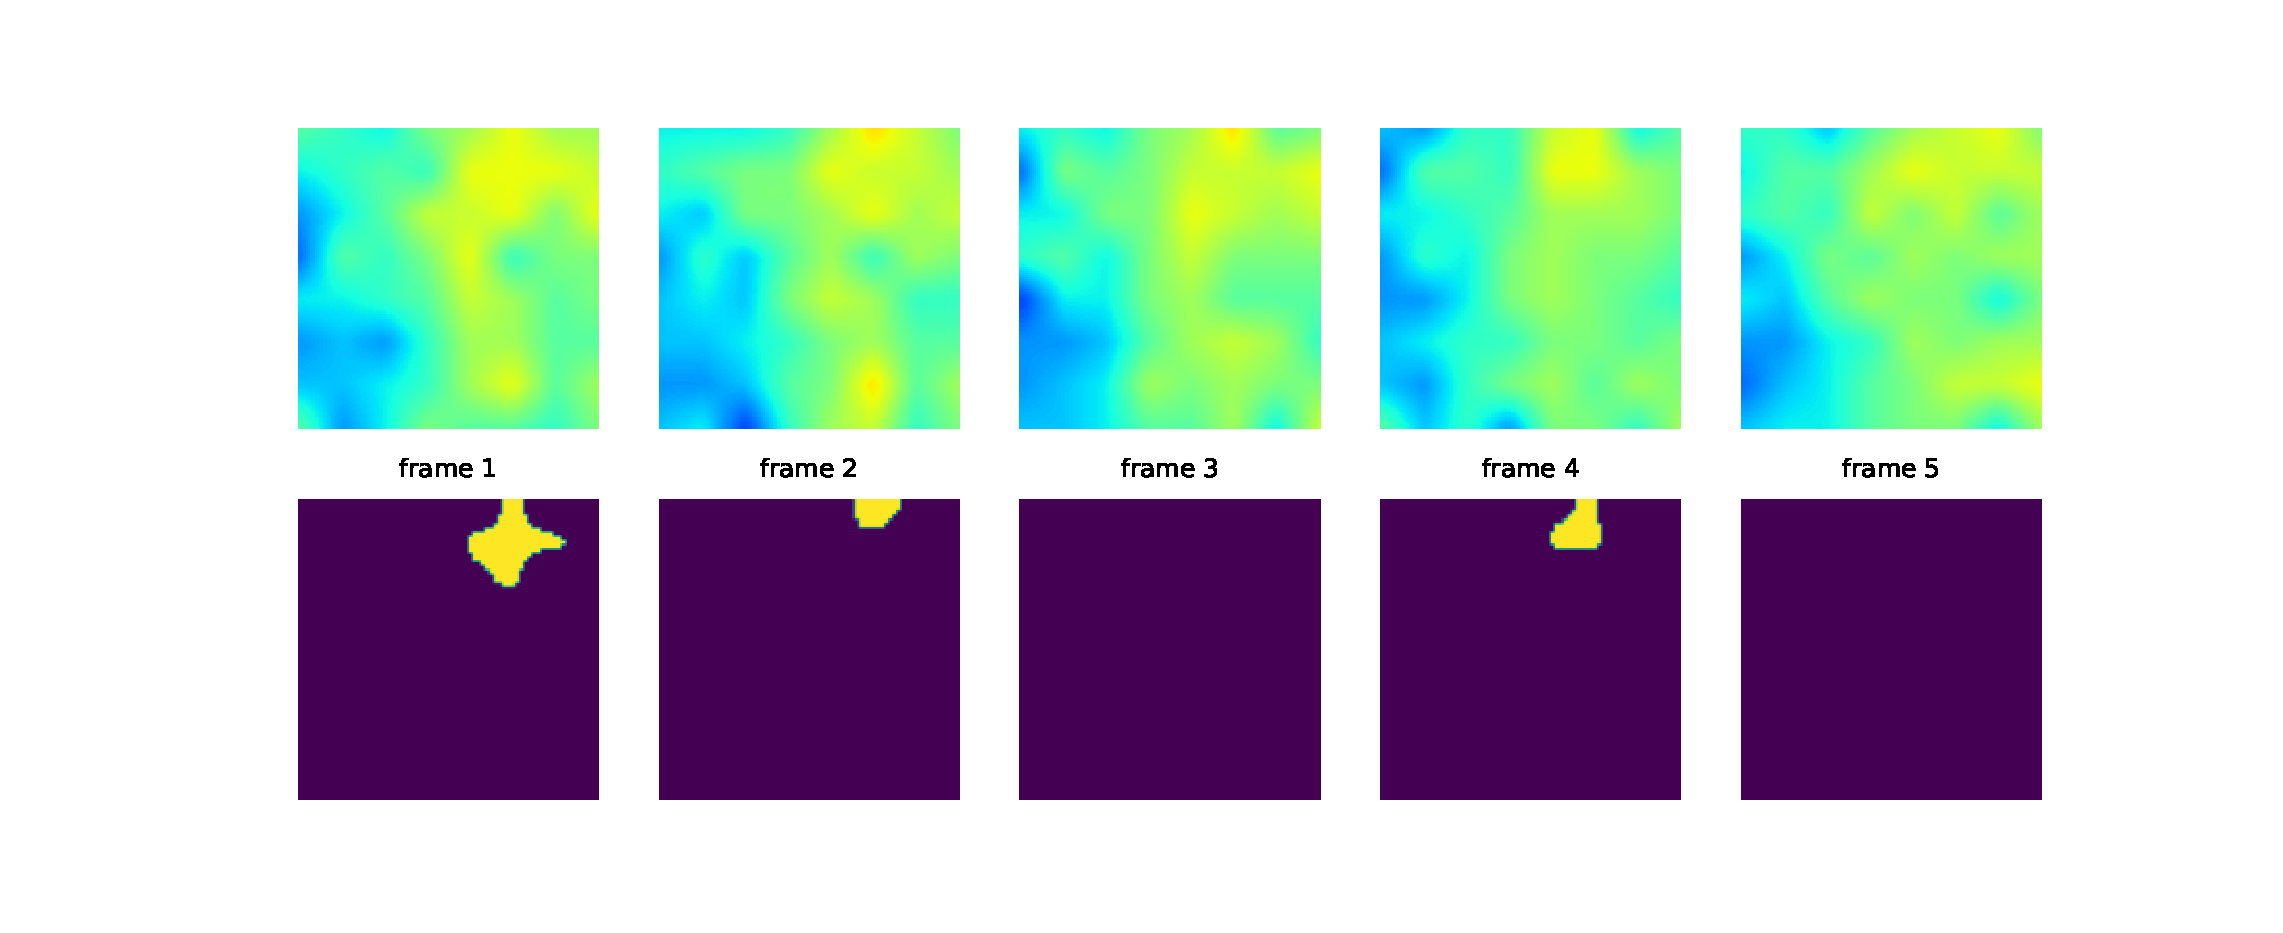
\includegraphics[width=\textwidth]{figures/err_noise1.eps}
  \caption{Sensor noises will not be tracked and counted even when they are incorrectly detected as objects because the sequence is usually not coherent.}\label{fig:err_no1}
\end{figure}
\begin{figure}
  \centering
  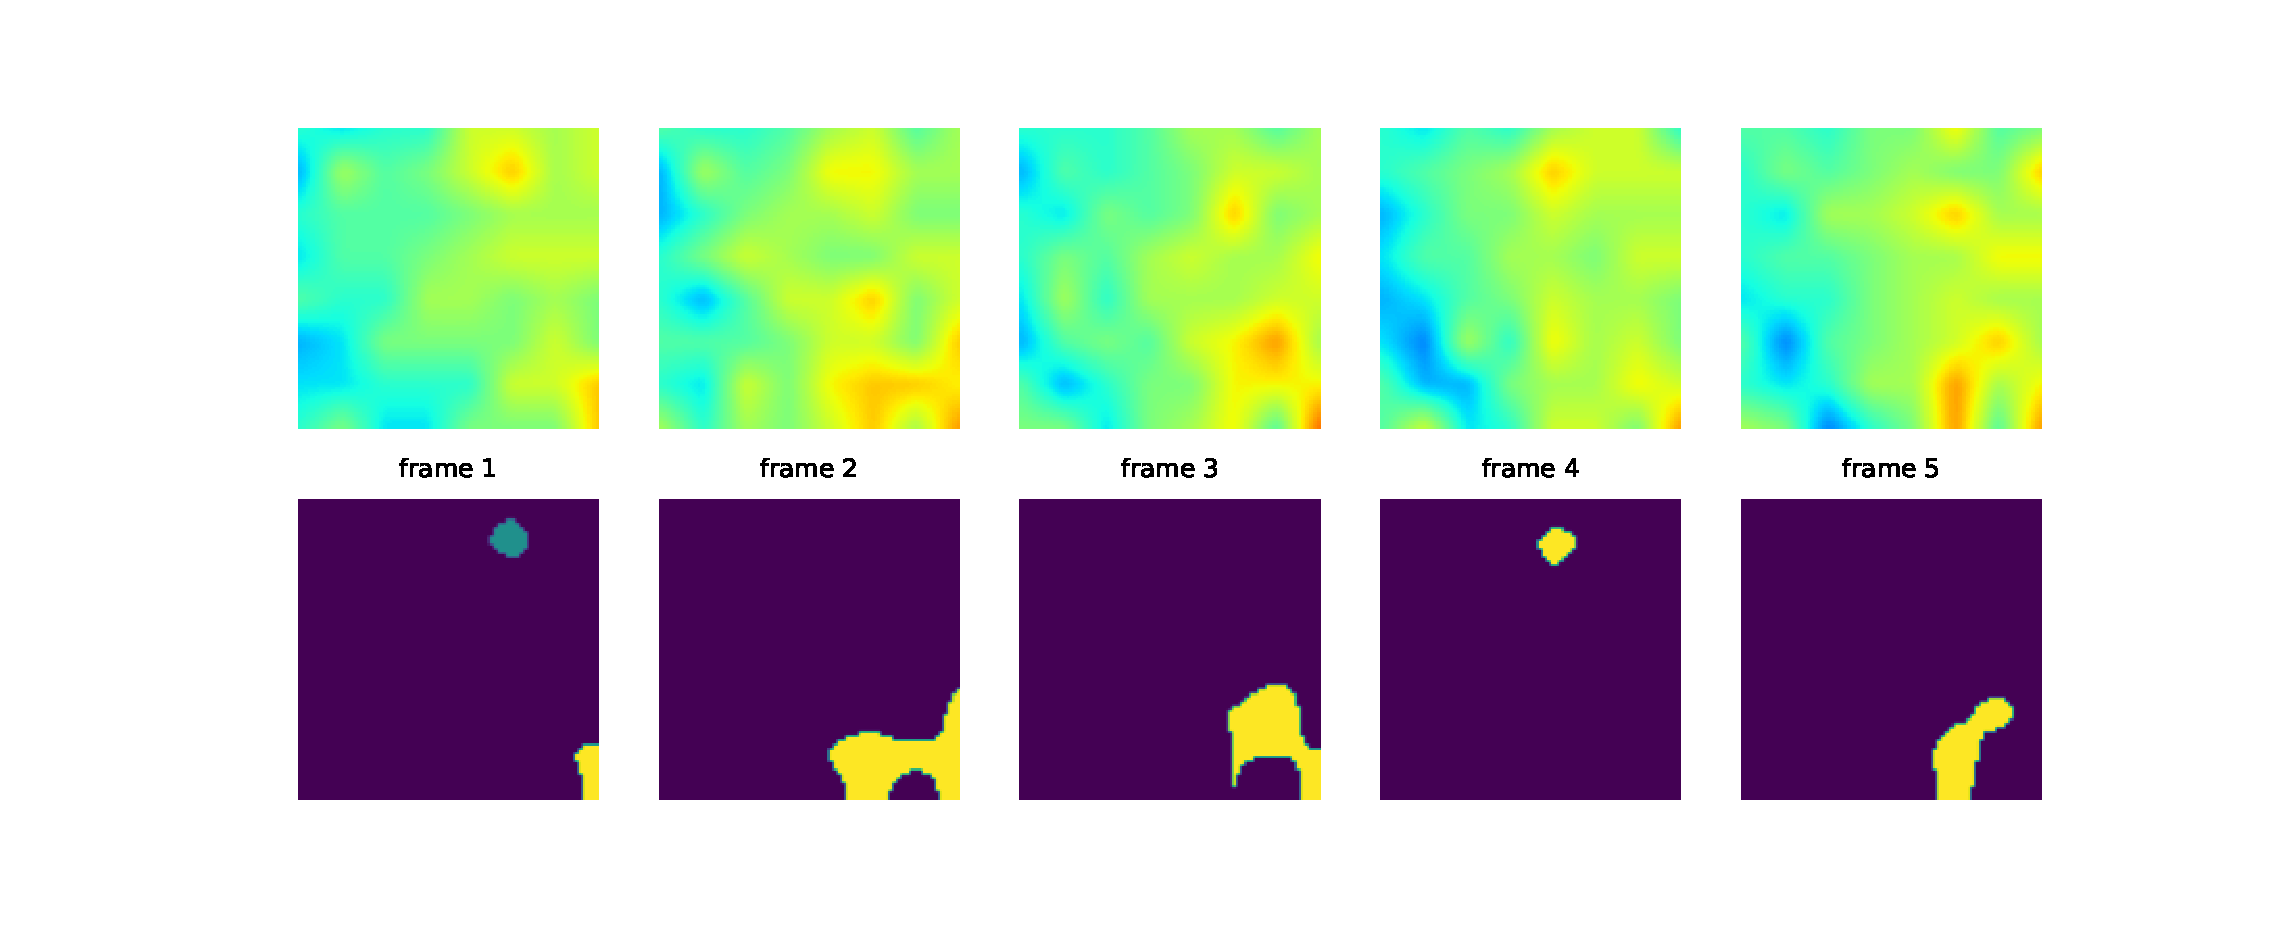
\includegraphics[width=\textwidth]{figures/err_noise2.eps}
  \caption{A noisy image sequence that may generate a wrong counting result. In the first 3 frames, the tracker has spawned an object in the right-bottom corner of the image. Later, the noise in frame 4 may be matched with the noise in frame 3, and the non-existing ``object'' has passed across the middle line. And in the next frame it disappears, which is considered as the termination of an exiting event. The human count is incorrectly decreased by one.}\label{fig:err_no2}
\end{figure}
Sometimes the temperature of a few pixels may temporarily exceed the segmentation threshold and be regarded as objects. The result is a few small objects emerging and disappearing randomly. We name this anomaly ``noise''. \autoref{fig:err_no1} shows an example of a noisy sequence. Fortunately, sensor noises usually will not cause a problem because they do not have an enter or exit tendency pattern as humans do. Tracking of a false detected noise pixel will fail within one or two frames and do not have an impact on the counting result. The only drawback is that the device will send too many rubbish messages to the storage platform if the camera is frequently activated by noises, which brings about the difficulty in debugging. Nevertheless, there are some noise sequences that cause a malfunction in the tracker, see \autoref{fig:err_no2}. When two noise trunks happen to emerge sequentially at different sides of the middle line, the tracking algorithm will take them as two frames of a moving object and generates incorrect results. Interestingly, we found that most of the problematic noisy sequences take place in the midnight when the ambient temperature drops. Therefore, the sensor noise issue should be traced back to the object detection layer. An improvement in \autoref{eq:detectionthreshold} may solve this problem.

Another potential issue takes place when a human stands under the camera for a long time, which is named as ``long sequence''. When there is an object in the camera view, the counting device needs to track it for every frame. The object must be segmented from the background over and over, the tracker needs to track the object even if it does not move at all, and the radio module keeps sending messages in minutes, which results in a lot of waste of computation power. Moreover, if a human occupies a certain area in the camera view, it increases the chance of incorrect matching when another person passes by. We have observed 6 long sequence anomalies during the real situation evaluation and all of them have been handled correctly.

Finally, the ``not detected'' issue describes when a human object passes under the camera but is not detected. This may happen when the human body temperature is too low, either because the body is covered by clothes or the person is short (the distance between camera and body enlarges for a short person, thus a lower detected body temperature). This issue can be solved by switching to a better IR camera with a larger detection range. It is also worth mentioning that the device only sends raw IR images for ground truth annotation when there are at least three pixels hotter than the room temperature. Therefore it is very likely that more events are not detected but also not noticed at all. This system bias in our experiment design can be solved by introducing another counting device based on different principles as a reference, for example, light barriers. An RGB camera may also help in collecting the ground truth if the privacy violation issue is lifted.

\section{Power Consumption}
The power consumption of the whole device is also an important aspect of the evaluation. The DHT11 temperature sensor consumes 1mA when measuring and 150µA when standby. The AMG8833 IR camera should run constantly and its average consumption is 4.5mA. \autoref{tab:esp32_power} shows the current consumption of the ESP32 in different modes. Without any power-saving tricks, the microcontroller consumes around 30mA (clock rate 160MHz) when idle and around 200mA when a human passes by. Assuming there are 40 enter and exit events every day and each event lasts 4 seconds (from image capturing until message publishing), the daily power consumption can be calculated approximately by \autoref{eq:power_estimate1}. On a common 600mAh Lipo battery, the device can operate for 16.5 hours, which is unsatisfying for an IoT application.
\begin{equation}\label{eq:power_estimate1}
\begin{split}
  P = (I_{esp32\ idle}+ I_{dht11}+I_{camera})mA * 24 hours + I_{esp32\ active}* t *n\\ \approx 852mAh +  9mAh = 860mAh
\end{split}
\end{equation}

It can be observed that though the radio module consumes the highest peak current, most of the battery power is wasted during the idle time because the device has to monitor the doorway all the time. To prolong the battery life, the key is how to reduce the power consumption when there is no event. Fortunately, Espressif provides many low-power options that can be integrated into our project. The light sleep mode can clock-gate the CPU and resume when an interrupt is triggered in the RTC peripheral. The deep sleep mode can power off the CPU totally to drastically reduce the power consumption lower than 1mA. Moreover, there is an 8MHz ultra-low-processor (ULP) along with the dual-core CPU that can retrieve sensor state and do some basic calculations when the main processors enter sleep mode, it can also wake up the main processors when necessary.

The power-saving design of our project contains two phases. The idle phase mainly contains the active pixel detection, i.e. the camera is polled by the ULP every 100ms to check if there is any pixel hotter than the environment temperature. And in the active phase, the ULP hands over the control of the camera to the main processors to track the object. To ensure an instant response of the human monitor device, we choose the light sleep mode because power up the main processors from deep sleep takes at least one second. Furthermore, we can neither afford the overhead of establishing the network connection whenever the main processor wakes up, so the RF module is kept powered on during sleep time. This results in power consumption of around 5mA during idle time. With the new idle current consumption, the daily consumption of the device is reduced to around 240mAh, and it can last around 2.5 days on a 600mAh battery.

More power is saved by deactivating the radio module so that the light sleep mode can be fully exploited. A constant network connection is required because the image data are too large to store in the internal memory, therefore we need to publish messages instantly. However, the image data are merely published for evaluation purpose and our algorithm works without the stored images. Without the image data, messages can be buffered in the memory and only send out once every hour. By this way we only bear the high current consumption during the relative short publish period and spare the expensive maintenance of the network. The estimated daily power consumption by this design is about 140mAh, see \autoref{eq:power_estimate2}. 
\begin{equation}\label{eq:power_estimate2}
\begin{split}
  P = (I_{esp32\ idle}+I_{camera})mA * 24 hours + I_{esp32\ active}* t_{event} *n \\+ I_{esp32\ publish}*t_{publish}*24\\ 
  \\\approx (1mA+ 4mA) * 24 hours + 40mA * (4s/3600) hours * 40 \\+ 180mA * 10s * 24
  \\= 120mAh +  8mAh + 12 = 140mAh
\end{split}
\end{equation}

By introducing additional sensors to detect approaching humans, the camera module no longer needs to operate constantly, which saves more power. For example, PIR sensors can be installed at both directions of the doorway to wake up the counting device in advance.   
The battery life can be further prolonged by deliberately shut down the device during midnight when it is unlikely to have any event.

\begin{table}[]
\centering
\begin{tabular}{|l|l|l|}
\hline
\textbf{Power mode}                  & \textbf{Description}            & \textbf{Power consumption} \\ \hline
Active (RF working)         & Wi-Fi transmit 802.11n & 180mA             \\
                            & Wi-Fi receive 802.11n  & 95 $\sim$100mA    \\ \hline
Active (RF not working)     & dual core 240MHz       & 30mA $\sim$68mA   \\
                            & dual core 160MHz       & 27mA $\sim$44mA   \\
                            & dual core 80MHz        & 20mA $\sim$31mA   \\ \hline
Light sleep with RF working & -                      & 5mA               \\
Light sleep                 & -                      & 0.8mA             \\ \hline
Deep sleep                  & ULP powered on         & 150µA             \\ \hline
\end{tabular}\caption{Power consumption of ESP32-WROVER module in different modes. The values are given by the ESP32 datasheet \cite{esp32datasheet} and confirmed by actual measurements.} \label{tab:esp32_power}
\end{table}

\section{Limitations}
The proposed algorithm has a few fundamental shortages. First of all, the object detection phase strongly depends on an accurate room temperature measurement and has a deterministic influence on the tracking result as the segmented object is the base of the following steps. Besides, the tracking algorithm based on central points can only handle multi-human events up to three or four people, if they were separated in the first few frames. The central point representation won't reflect the truth in crowded scenarios because multiple people will be regarded as one, for example, a large number of people crowding at the doorway when a meeting ends. Furthermore, our algorithm can not track a human who runs through the doorway, because the nearest neighbor matching method assumes the largest matching radius that is calculated from common walking speed.

There are also limitations to hardware. Currently, it takes around 20ms to process a single frame at a 160MHz CPU clock rate. The processing time may be longer if switching to a low-end MCU and eventually exceeds the time constraint. The program requires 953KB Flash and 220KB memory, the large memory requirement is mainly because of the image interpolation step. For images smaller than $71\times71$ resolution, the memory usage will likely remain the same. For larger images, both memory usage and process time will increase. 